%\documentclass[twocolumn]{scrartcl}
\documentclass[DIV=14,twocolumn]{scrartcl}
\usepackage[pdftex]{hyperref}
\usepackage{cite}
\usepackage{amsmath}
\usepackage{amssymb}
\usepackage[]{algorithm2e}
\usepackage{graphicx}

\DeclareMathOperator{\rank}{rank}
\newcommand{\norm}[1]{\left\lVert#1\right\rVert}

%opening
\title{Report over statistical learning theory lab final project}
\subtitle{Building a recommender system with matrix factorization}
\author{Markus Fischer\\ \small{\href{mailto:markus.fischer@uni-jena.de}{markus.fischer@uni-jena.de}}}
\date{25.07.2019}

\begin{document}

\maketitle
\begin{abstract}
Abstract comes later
\end{abstract}

\section{Task and Dataset}\label{intro}
To pass the course "Statistical Learning Theory Lab" we were required to write a recommender system as final project. There are two ways to interpret this task.
The first, less technical interpretation is the following: Roughly speaking, we want to predict the rating $\hat{r}_{u,i}$ that some user $u$ might give to a item $i$, depending on the previous ratings of this user or item.

With a more technical point of view, our task is to complete a highly sparse matrix. The original ratings are composed in a matrix $R\in\mathbb{R}^{m\times n}$ where the rows represent the $m$ users and the $n$ columns the items.
Each entry $r_{u,i}$ then stands for the rating of user $u$ for item $i$. We now want compute a dense matrix $\hat{R}$ were we assign a rating for each user-item pair.

There are many approaches to do this. In \cite{KoBeVo09} two of the most common algorithms for this task are described.
One approach follows the assumption similar users rate items similarly. Such algorithms try to determine the distance between two users or items and then use a $k$-Nearest-Neighbor algorithm to compute the rating depending on their ratings.

The second common approach is often called latent factor model. The idea is the following: each item belongs to certain concepts. Each user may like some of these concepts more than others. In the world of films that could be the genre of the movie. A latent factor approach now tries to explain the ratings of items with respect to this categories. Usually they compute a decomposition of the ratings matrix.

\subsection{Dataset Insights}\label{datsetinsight}
We got a set of 461,806 triples of the form (row, column, rating) and we were required to rate another 81,495 row-column pairs. 
The given training data stretch out to matrix of the dimension $5499\times 2080$. Since this matrix has 11,437,920 possible entries we have around $95.9\%$ sparsity.

Our ratings are in the set $\{0,1,2,3,4\}$. Since 0 is a possible rating it is useful to apply a feature map $$\phi:\mathbb{N}\rightarrow\mathbb{N},m\rightarrow m+1$$ before any other computation. As a result we can assume that 0 in our ratings matrix stands for an empty field and not for the rating 0. To get our final, correct ratings we should apply the inverse feature map $\phi^{-1}$ as final step.

\subsection{Item and User Bias}\label{bias}
Let us look a bit deeper in our dataset. As a first step let us compute the distribution of the number of ratings for items. As you can see in \autoref{fig:itemcount}, around one half of the items were rated by users. Most of the rated items received at least 300 ratings. 
\begin{figure}[h]
	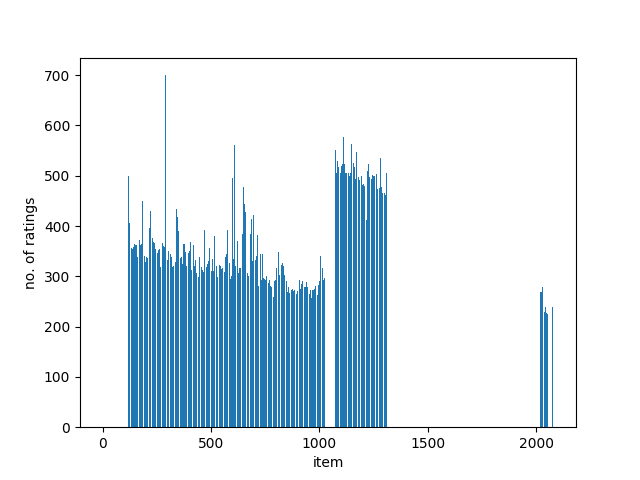
\includegraphics[width=\columnwidth]{../img/item-count}
	\caption{rating count per item}
	\label{fig:itemcount}
\end{figure}

More interesting is the distribution of ratings per user. When we look on \autoref{fig:usercount}, we can see that there exist some users that rate around one half of the items. On the other hand a majority of users rate only a few items. We can safely say, that there exist a large bias for some users. As a consequence we need to incorporate this bias in our models to improve our prediction.
Since some of the items are also rated more often, there exist a item bias as well. 
\begin{figure}
	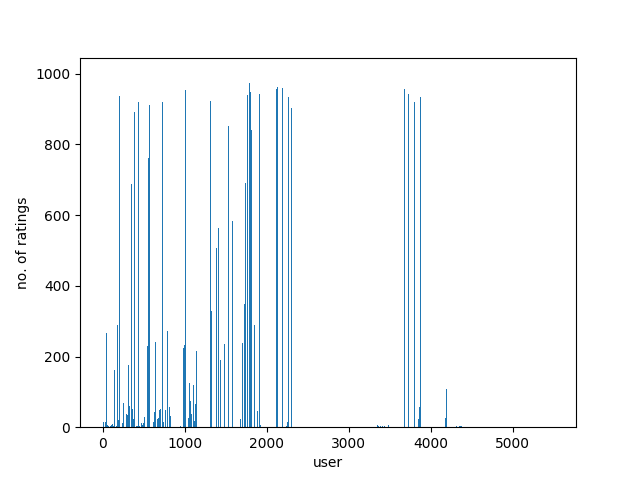
\includegraphics[width=\columnwidth]{../img/user-count}
	\caption{rating count per user}
	\label{fig:usercount}
\end{figure}

\section{Measuring the Performance}
To compare variants of our model and select the best one, it is necessary to have a objective measure. There are many different metrics for this. It depends on our concrete task which one we should consider. In our case only the accuracy of the system is interesting.

One common metric to measure the accuracy of a predictor is the root mean square error (RMSE). Let $r_{u,i}$ be the observed rating, $\hat{r}_{u,i}$ the predicted rating and let $n$ be the number of predictions. Then the RMSE is defined in the following way: 
\begin{equation*}
\begin{split}
\text{RMSE} = \sqrt{\frac{\sum_{\text{predicted ratings}} (r_{u,i}-\hat{r}_{u,i})^2}{n}}
\end{split}
\end{equation*}
This is a measure of how good our model fit the given dataset. Keep in mind, that this measure tends to disproportionately penalize large errors. 

For more metrics refer to \cite{Ag16}.

\section{Baseline Predictors}\label{baseline}
To get a feeling of the dataset it is useful to implement very basic baseline predictors. For example we could use the mean of the ratings specified by user $u$ to specify a new rating $\hat{r}_{u,i}$ for item $i$. In an analogue way we could use the mean of an item $i$ for new ratings. A third option is the usage of random values. 

\begin{table}[h]
	\centering
	\begin{tabular}{r|l}
		method & RMSE \\ \hline
		user mean & 0.700 \\
		item mean & 0.772 \\
		random & 1.780
	\end{tabular}
	\caption{RMSE for baseline models}
	\label{tab:baseline}
\end{table}

If we split our given dataset in a training set and in a test set and using the above described methods lead to the results stated in \autoref{tab:baseline}. The value for the random method, was determined after one run. Repeating this experiment might give other values.

We notice that the mean methods already give us quite good results. The better result of the user mean model can be explained with the in \autoref{bias} described bias. Models that are above these values can be easily ignored. 


\section{Matrix Factorization}\label{matrixfactorization}
A better way to solve such a task is the usage of matrix factorization techniques. The idea is the following: given is a ratings matrix $R\in\mathbb{R}^{m\times n}$. We assume that $\rank(R)=k\ll\min(m,n)$. Then this matrix can be decomposed in two smaller matrices such that 
$$R\approx UV^T$$ holds, where $U\in\mathbb{R}^{m\times k}$ and $V\in\mathbb{R}^{n\times k}$. This is an example for matrix factorization as described in \autoref{intro}.

As stated in \cite{KoBeVo09}, one common way to do this, is the usage of singular value decomposition (SVD), which works fine with dense matrices. In our case the matrix $R$ is highly sparse and SVD wouldn't work. Instead the problem can be reformulated as optimization problem, as described in \cite{Ag16}. We can use the following objective function: 
$$\min_{U,V} \frac{1}{2}\norm{R-UV^T}^2$$ 
$\norm{\cdot}^2$ refers here to the squared Frobenius norm which is defined as $$\norm{A}^2:=\sum_{i,j}A_{i,j}^2$$

In the easiest variant of such a optimization problem, we assume that there are no further constraints. We refer to this variant as unconstrained matrix factorization (UMF). 
It is common to compute the solution of this problem with gradient descent method.

\subsection{Gradient Descent}\label{gd}
The gradient descent method is an iterative approach to find an $x$ that minimizes a differentiable function $f$ starting with a given $x^{(0)}$. As a first step it is necessary to compute the gradient $\nabla f$ of the function, which points in the direction of the highest ascent. 
The idea to minimize the function is now going small steps in the opposite direction. An algorithm for this is described in \autoref{algo:gd}. 

\begin{algorithm}
	\caption{gradient descent}
	\label{algo:gd}
	\KwData{starting point $x^0$, learning rate $\eta > 0$}
	\KwResult{$x$ that minimizes $f$}

	\While{no convergence}{
		calculate $\nabla f$\;
		update $x^{(n+1)} \leftarrow x^{(n)} - \eta \nabla f$ \;
	}
\end{algorithm}
Note that this is only the easiest example for gradient descent methods. Keep in mind, that for a to large $\eta$ the algorithm shows divergence.
For an more detailed description refer to \cite{ShSh14}. 

\subsection{Applying Gradient Descent on UMF} 
We want to apply the gradient descent approach on the unconstrained matrix factorization problem. 
As a first step it is necessary, to calculate the gradient of our objective function. There are only a few observed entries in the ratings matrix $R$. The objective function is therefore undefined. To fix this it is necessary to set the unobserved entries in $UV^T$ and $R$ to zero. This works only if we applied the feature map $\phi$ given in \autoref{datsetinsight}. 
Now let us define $E:=R-UV^T$ as the error matrix. Again all unobserved entries in this matrix are zero, and don't affect the loss function. Our objective function becomes now \[\min\frac{1}{2}\norm{E}^2\]
With this in mind, we can calculate the gradient of our objective function.
Let us start with respect to an entry in matrix U.
\begin{equation*}
\begin{split}
\nabla_{U_{i,\beta}} \frac{1}{2}\norm{E}^2 &= \nabla_{U_{i,\beta}} \frac{1}{2}\sum_{i,j}E_{i,j}^2 \\ &=\nabla_{U_{i,\beta}} \frac{1}{2}\sum_{i,j}(R_{i,j}-(UV^T)_{i,j})^2 \\
&=\nabla_{U_{\alpha,\beta}} \frac{1}{2}\sum_{i,j}(R_{i,j}-\sum_{l=1}^k U_{i,l}V^T_{l,j})^2\\
&=\sum_{i,j}(R_{i,j}-\sum_{l=1}^k U_{i,l}V^T_{l,j})(-V^T_{\beta,j})\\
&=\sum_{i,j}(E_{i,j})(-V_{j,\beta})=-EV_{i,\beta} 
\end{split}
\end{equation*}
It is possible to derive the gradient for an entry in matrix V symmetrical. We get 
\begin{equation*}
\begin{split}
\nabla_{V_{j,\alpha}} \frac{1}{2}\norm{E}^2 &= \nabla_{V_{j,\alpha}} \frac{1}{2}\sum_{i,j}(R_{i,j}-(UV^T)_{i,j})^2\\
&=\sum_{i,j}(E_{i,j})(-U_{i,\alpha})=-E^TU_{j,\alpha}
\end{split}
\end{equation*}

Those gradients can be easily vectorized to $$\nabla_U \frac{1}{2}\norm{E}^2=-EV$$ and  $$\nabla_V \frac{1}{2}\norm{E}^2=-E^TU$$. Since the learning rate $\eta$ needs to be positive we get the following update rules: \[U^{(i+1)} \leftarrow U^{(i)} + \eta E^{(i)}V^{(i)}\] and \[V^{(i+1)} \leftarrow V^{(i)} + \eta E^{(i)T}U^{(i)}\]
For minimizing the objective function with \autoref{algo:gd}, it is necessary to have a starting point. One option to obtain $U^{(0)}$ and $V^{(0)}$ is the initialization with random values. 

As a last thing, it is necessary to have a convergence criteria or our algorithm runs in a infinite loop. One possibility is that the value of our objective function should be below a certain value. But since the gradient descent finds a local, previously unknown, minimum it is hard to decide when to stop. It is therefore better to use other criteria. In my implementation I stop when the difference of the objective function value between two iterations is below a certain limit. Formally the algorithm stops when
\begin{equation*}
\begin{split}
&|\frac{1}{2}\norm{E^{(n)}}^2-\frac{1}{2}\norm{E^{(n+1)}}^2|=\\
&\frac{1}{2}|\sum_{i,j}(E_{i,j}^{(n)})^2-(E_{i,j}^{(n+1)})^2|\leq\epsilon
\end{split}
\end{equation*} $$$$ holds.

\textit{Note:} It is also possible to reshape the matrices in vectors of the dimension $(mk)\times1$ and $(nk)\times1$. 

\subsection{Regularization to Prevent Overfitting}
In order to prevent overfitting it is common to add a regularization term to the objective function. As stated in \cite{Gi19} this may increase the bias but it also may decrease the variance of the estimator. This is known as bias-variance trade-off and can lead to a better predictor. 

For our matrix factorization problem we can  add the regularization terms $\frac{\lambda}{2}\norm{U}^2$ and $\frac{\lambda}{2}\norm{V}^2$ for $\lambda \geq 0$ as recommended in \cite{Ag16}.
Plugging this into the objective function give following problem: $$\min_{U,V} \frac{1}{2}\norm{E}^2 + \frac{\lambda}{2}\norm{U}^2 + \frac{\lambda}{2}\norm{V}^2$$. Calculating the gradient of this objective function gives two, a bit modified update rules: \[U^{(i+1)} \leftarrow U^{(i)} + \eta E^{(i)}V^{(i)} - \eta\lambda U^{(i)}\] and \[V^{(i+1)} \leftarrow V^{(i)} + \eta E^{(i)T}U^{(i)} - \eta\lambda V^{(i)}\]
Setting $\lambda = 0$ gives the original problem with no regularization. It is therefore possible to use these update rules even in the unregularized case.
\subsection{Incorporating Bias}
Users and items are different. Some users may rated many items and others only a few. And some items are bought more often then others and therefor they may have more ratings. We have seen this problem in \autoref{datsetinsight}.
 
The first step to encounter this problem it is useful to mean center our original matrix with the global mean $\mu$. If this is done it is necessary to add the mean after the calculation of our ratings.

As described in \cite{Ag16} it is possible to improve this even more. Let us associate with each user $i$ a variable $o_i$ which indicates the bias of user $i$ to rate items. Users who rate items high or more often might have a high value, users who rate very rarely items may have small (negative) values. Vice versa we can introduce a similar variable $p_j$ for items.
 
Our predicted rating for items become now $$\hat{R}_{u,i} = \mu + o_u + p_i + UV^T_{u,i}$$. Our error matrix becomes now $$E_{u,i} = R_{u,i}^{'} - \hat{R}_{u,i} = R_{u,i}^{'} - o_u - p_i - UV^T_{u,i}$$. Note that $R^{'}$ denotes the mean centered data matrix and as a result $\mu$ plays no role in the following calculations.

Now let us look at the following equation:
\begin{equation*}
\begin{split}
o_u + p_i + UV^T_{u,i} &= \sum_{l}^{k}U_{u,l}V^T_{l,i} + o_u + p_i\\ &= \sum_{l}^{k}U_{u,l}V^T_{l,i} + o_u\cdot 1 + 1\cdot p_i
\end{split}
\end{equation*}
It is easy to see that the last two terms can added to the sum if we increase $k$ by $2$ and set $U_{u,k+1}=o_u$ and $V^T_{k+1,i}=1$ as well $V^T_{k+2,i}=p_i$ and $U_{u,k+2}=1$. Our new problem is now nearly similar to our original problem. The only difference is now, that there exist two new small constraints. The column $k+2$ in $U$ and the column $k+1$ in $V$ must be $1$.
These constraints can be satisfied in the gradient descent approach if we set these columns after each update step to $1$ as described in \cite{Ag16}.

\subsection{Improving the Gradient Descent}
We have seen that the gradient descent is one method to minimize our optimization problem. But as described in \ref{gd} for to large $\eta$ the algorithm shows divergence.
On the other hand for to small $\eta$ the algorithm needs many cycles for convergence. Therefor the algorithm give us room for improvements.

One common way is the usage of stochastic gradient descent SGD. This is the recommended way in \cite{KoBeVo09}. The idea is not to use the gradient of our objective function but an random vector which expected value lies in the (sub-)gradient of the function. For a detailed description refer to \cite{ShSh14}.

We want to use another way. Let us stick with the gradient descent but let us choose $\eta$ in a way that it should be large enough to minimize the function fast but small enough to show no divergence. 

Since we are using a iterative approach the best $\eta$ would be the one, that minimizes $\psi(\eta) = f(x-\eta\nabla f(x))$ for $\eta > 0$. The brute-force algorithm would perform a linear search on $\eta$. But as you notice this is computational expensive.  But there exist some numerical methods to find such $\eta$ in relative fast time. For example such $\eta$ could met the Wolfe conditions:
\begin{equation*}
\begin{split}
f(x-\eta\nabla f(x)) \leq f(x) + c_1\eta\nabla f^T\nabla f(x)
\end{split}
\end{equation*}
\begin{equation*}
\begin{split}
\nabla f(x-\eta\nabla f(x))^T\nabla f(x) \geq c_2\nabla f^T\nabla f(x)
\end{split}
\end{equation*}
for $0 < c_1 < c_2 < 1$.
With this there exists some numerical faster algorithms as described in \cite{NoWr06}.

With this approach we can use our algorithm. The computation of $\eta$ needs now more time but since the step size fits now better we need much less cycles and therefor our algorithm may converge faster. 

Note the following. Since $\eta$ is not fixed it is not sure that $|\frac{1}{2}\norm{E^{(n)}}^2-\frac{1}{2}\norm{E^{(n+1)}}^2|$ gets smaller for every iteration. Sometimes the improved algorithm does big steps. But our convergence criteria works since the steps will be get asymptotically smaller. Also the objective function value gets smaller from iteration to iteration. 

\section{Model Evaluation And Parameter Tuning}
The in \autoref{matrixfactorization} described model has two main parameters. The most important is the rank of the decomposition matrices. The second interesting parameter is the regularization parameter $\lambda$. It would also be interesting to see the impact of the bias variables.

For the following experiment the given data set was splitted in two halfs. 90\% of the dataset were used for training. The remaining 10\% were used to calculate the RMSE. 

Since the rank of the matrix has more impact on the result it is useful to start the search there. I trained 5 models with rank 1 to 20 in steps of five. I used constant $\eta=0.0005$, no regularization and the convergence criteria $\epsilon = 0.001$. The maximum cycle count was set to 5000. To see a impact of the bias variables I repeated the experiment with the same parameters but incorporated bias.   
\begin{figure}[h]
	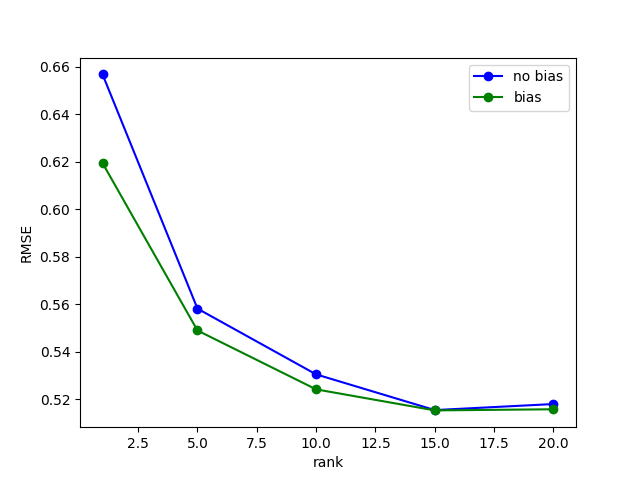
\includegraphics[width=\columnwidth]{../img/rank-rmse-validate}
	\caption{RMSE vs. matrix rank}
	\label{fig:ranksearch}
\end{figure}
The result of this experiments are shown in \autoref{fig:ranksearch}. Compared with our baseline models of \autoref{baseline} even the model with rank 1 works better. The performance of our model increase til rank 15. It is noticeable that the performance increase of our model gets slower. Between rank 15 and rank 20 the unbiased estimator performance get worse again. This might be a sign for overfitting. 
It is also worth to mention that the incorporation of bias has a huge impact on low rank models. With increasing rank the influence of the bias variables vanish increasingly. At rank 15 they have nearly no impact.
But on the other side it seems that biased estimators tend to overfit less.
\begin{figure}[h]
	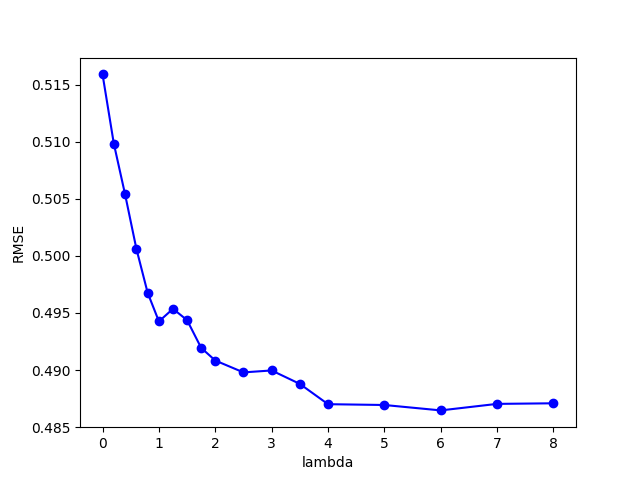
\includegraphics[width=\columnwidth]{../img/lambda-rmse-validate}
	\caption{RMSE vs. regularization parameter $\lambda$}
	\label{fig:lambdasearch}
\end{figure}

The regularization parameter has less impact on our model. 
\section{Conclusion}
\bibliography{references}{}
\bibliographystyle{alpha}
\end{document}
